\subsection{Example \#3 -- receiving test messages}
Let's simulate $n$ days, and in each one count the number of messages, if they arrive independently from a Poisson distribution with rate=10. In each day we count messages over 12 hours, so notice that how we multiply by 12 in the code below.

\begin{knitrout}
\definecolor{shadecolor}{rgb}{0.969, 0.969, 0.969}\color{fgcolor}\begin{kframe}
\begin{alltt}
\hlstd{ssize} \hlkwb{<-} \hlkwd{c}\hlstd{(}\hlnum{5}\hlstd{,}\hlkwd{seq}\hlstd{(}\hlnum{10}\hlstd{,}\hlnum{1000}\hlstd{,}\hlkwc{by}\hlstd{=}\hlnum{10}\hlstd{))}
\hlstd{myMsg} \hlkwb{<-} \hlkwd{rep}\hlstd{(}\hlnum{0}\hlstd{,}\hlkwd{length}\hlstd{(ssize))}
\hlkwd{set.seed}\hlstd{((}\hlnum{40001}\hlstd{))}
\hlkwa{for} \hlstd{(i} \hlkwa{in} \hlnum{1}\hlopt{:}\hlkwd{length}\hlstd{(ssize)) \{}
    \hlstd{myMsg[i]} \hlkwb{<-} \hlkwd{mean}\hlstd{(}\hlnum{12}\hlopt{*}\hlkwd{rpois}\hlstd{(ssize[i],} \hlnum{10}\hlstd{))}
\hlstd{\}}
\hlkwd{plot}\hlstd{(ssize, myMsg,}\hlkwc{pch}\hlstd{=}\hlnum{17}\hlstd{,}\hlkwc{col}\hlstd{=}\hlstr{"blue"}\hlstd{,} \hlkwc{axes}\hlstd{=}\hlnum{FALSE}\hlstd{)}
\hlkwd{axis}\hlstd{(}\hlnum{1}\hlstd{);} \hlkwd{axis}\hlstd{(}\hlnum{2}\hlstd{)}
\hlkwd{abline}\hlstd{(}\hlkwc{h}\hlstd{=}\hlnum{12}\hlopt{*}\hlnum{10}\hlstd{,} \hlkwc{lwd}\hlstd{=}\hlnum{2}\hlstd{,}\hlkwc{col}\hlstd{=}\hlnum{2}\hlstd{)}
\end{alltt}
\end{kframe}\begin{figure}

{\centering 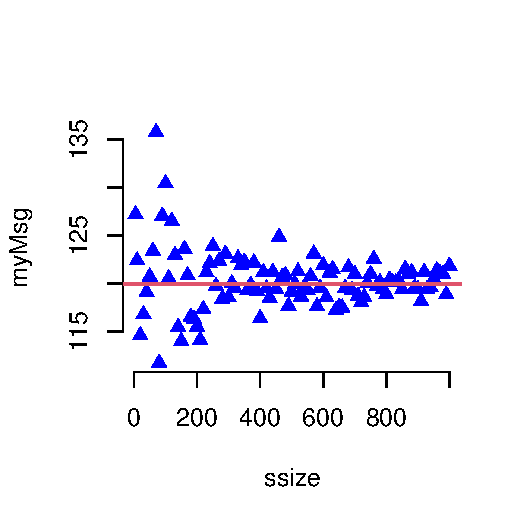
\includegraphics[width=\maxwidth]{figure/intro-lln2-0-1} 

}

\caption[Simulated text messages]{Simulated text messages.}\label{fig:intro-lln2-0}
\end{figure}

\end{knitrout}


If we continue to get text messages at this fixed rate over a long period of time, and we calculate the average daily messages (from 8am to 8pm) we see that that average converges to 12*10=120 messages per day. 
